\documentclass[unknownkeysallowed]{beamer}
\usepackage{graphicx}
\usepackage{multirow}
%\graphicspath{{images/}}


%\usepackage{pifont}


\usepackage{amssymb}
\usepackage{amsmath}
%\usepackage{booktabs}
%\usepackage{multirow}
%\usepackage{subfig}

\usepackage{tikz}

\pgfdeclareimage[height=2cm]{university-logo}{./images/shanghaitech-logo}
\logo{\pgfuseimage{university-logo}}

%\usebackgroundtemplate{%
%\tikz[overlay,remember picture] \node[opacity=0.3, at=(current page.center)] {
%   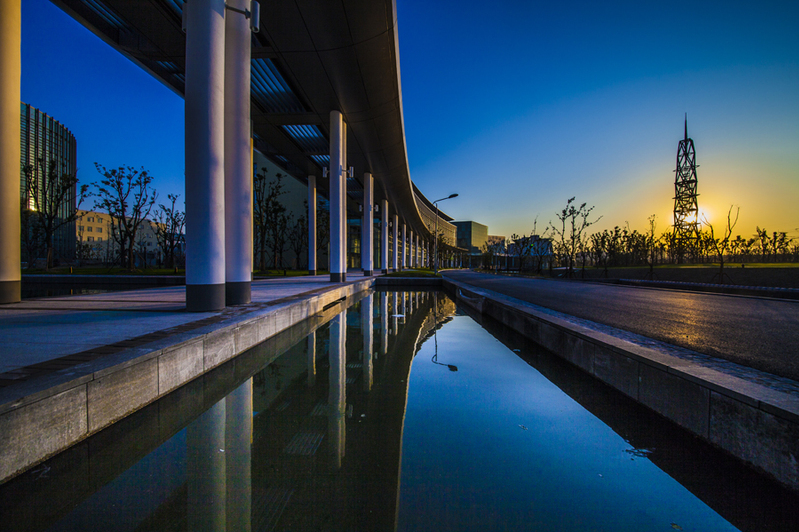
\includegraphics[height=\paperheight,width=\paperwidth]{images/shanghaitech_campus}};
%}

%\usebackgroundtemplate%
%{%
%    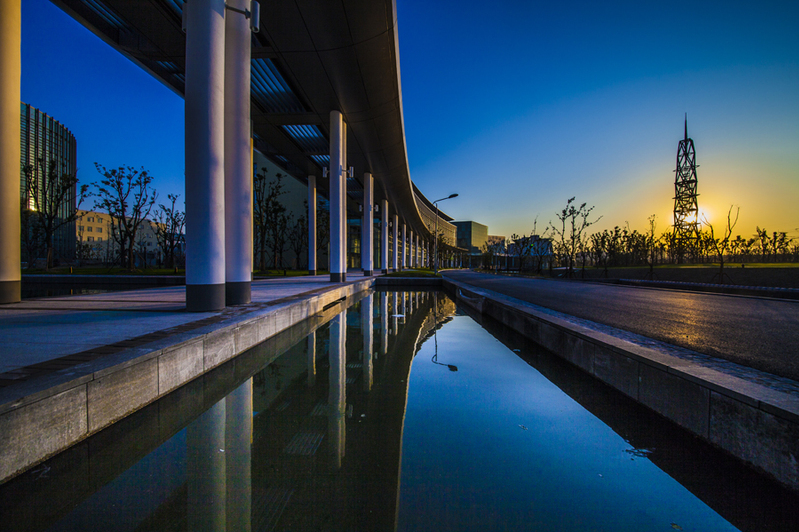
\includegraphics[width=\paperwidth,height=\paperheight]{images/shanghaitech_campus}%
%}

\usetheme{CambridgeUS}
%\usecolortheme{whale}

\title{Human Protein Image Classification}
\author[S.Y.Zhang\quad S.P.Yan\quad Y.F.Liu\quad B.Wan\qquad]{Songyang Zhang, Shipeng Yan,\\ Yongfei Liu, Bo Wan}

\institute
{
	School of Information Science and Technology \\
	ShanghaiTech University
}

\date{DIP Course Project, 2019}

%\AtBeginSubsection[]
%{
%	\begin{frame}<beamer>{Outline}
%%	\tableofcontents[currentsection,currentsubsection]
%	\tableofcontents[currentsection]
%	\end{frame}
%}

\begin{document}
	\begin{frame}
		\titlepage
	\end{frame}
	
	\begin{frame}
		\tableofcontents
	\end{frame}
	
%%%%%%%
% Section 1	Problem
% Subsection Background
%%%%%%%
 	\section{Problem}
	\subsection{Background}
	\begin{frame}{Background}
	
	\begin{columns}
		\begin{column}{0.3\paperwidth}
		\begin{figure}
			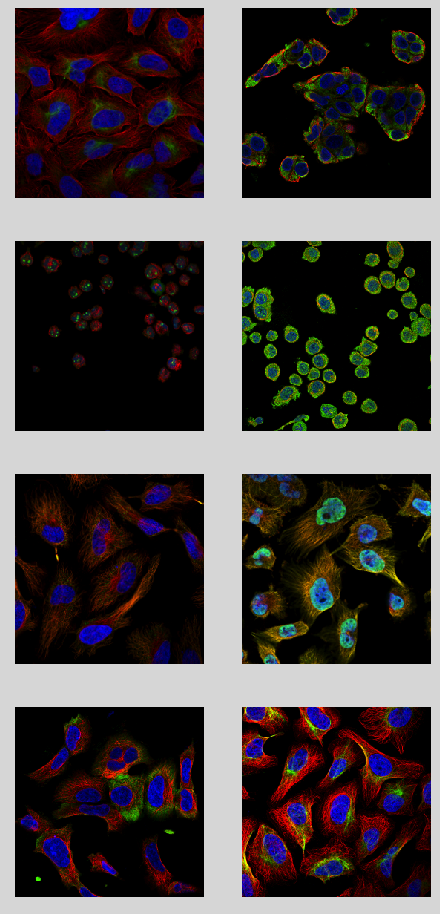
\includegraphics[width=0.25\paperwidth,height=0.6\paperheight]{images/background_1}
		\end{figure}
		\end{column}
		
		\begin{column}{0.7\paperwidth}
		\begin{block}{}
			\begin{itemize}
				\item Human protein classification can help us understand the human cells and disease.
				\item Classify mixed patterns across a range of different human cells is challenging
				\item High-throughput microscopy could generate high-resolution cell images.
				\item Human cells hold the key for the next breakthrough in medicine.
			\end{itemize}
		\end{block}
		\end{column}
	\end{columns}
	\end{frame}
	

%%%%%%%
% Section 1	Problem
% Subsection Terminology
%%%%%%%
	\subsection{Terminology}
	\begin{frame}{Terminology}
		\begin{block}{Problem Definition}
		Multi-label classification task requires the model give each input data multiple labels 
		\begin{itemize}
			\item Input: A 4-channel image $\mathcal{X}\in \mathbb{R}^{4*H*W}$, where $H$ and $W$ is the height and width of the image.
			\item Output: A subset of the label set $L \in Y, Y=\{y_1,y_2,\dots,y_n\}$, where $n$ is the number of category over the whole dataset.
			\item $0 \leq |L| \leq n$, $n=28$ in this task.
		\end{itemize}
		
		\end{block}
	\end{frame}

%%%%%%%
% Section 2	Method
% Subsection Data Analysis
%%%%%%%
	\section{Method}
	\subsection{Data Analysis}
	\begin{frame}{Data Analysis(1/3)}
		\begin{figure}
			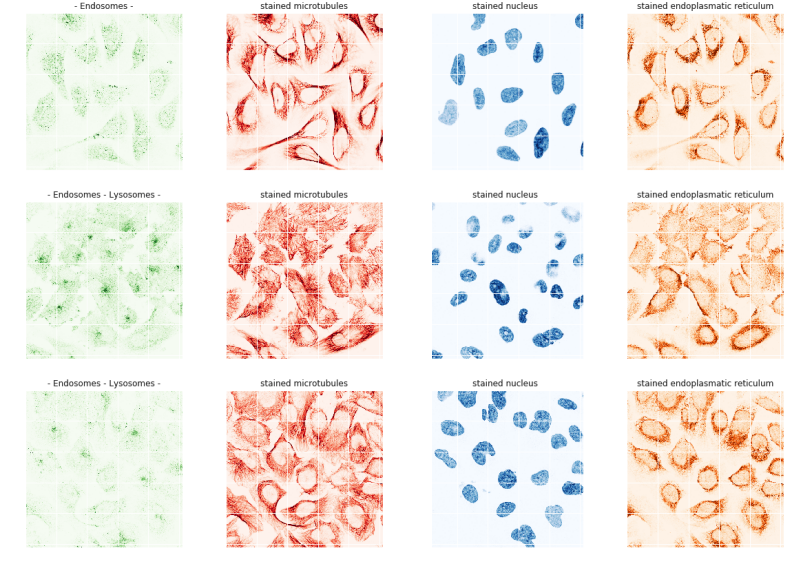
\includegraphics[width=0.8\paperwidth,height=0.8\paperheight]{images/data_analysis_0}
		\end{figure}
	\end{frame}
	\begin{frame}{Data Analysis(2/3)}
	\begin{block}{Target Correlation}
		\begin{figure}
			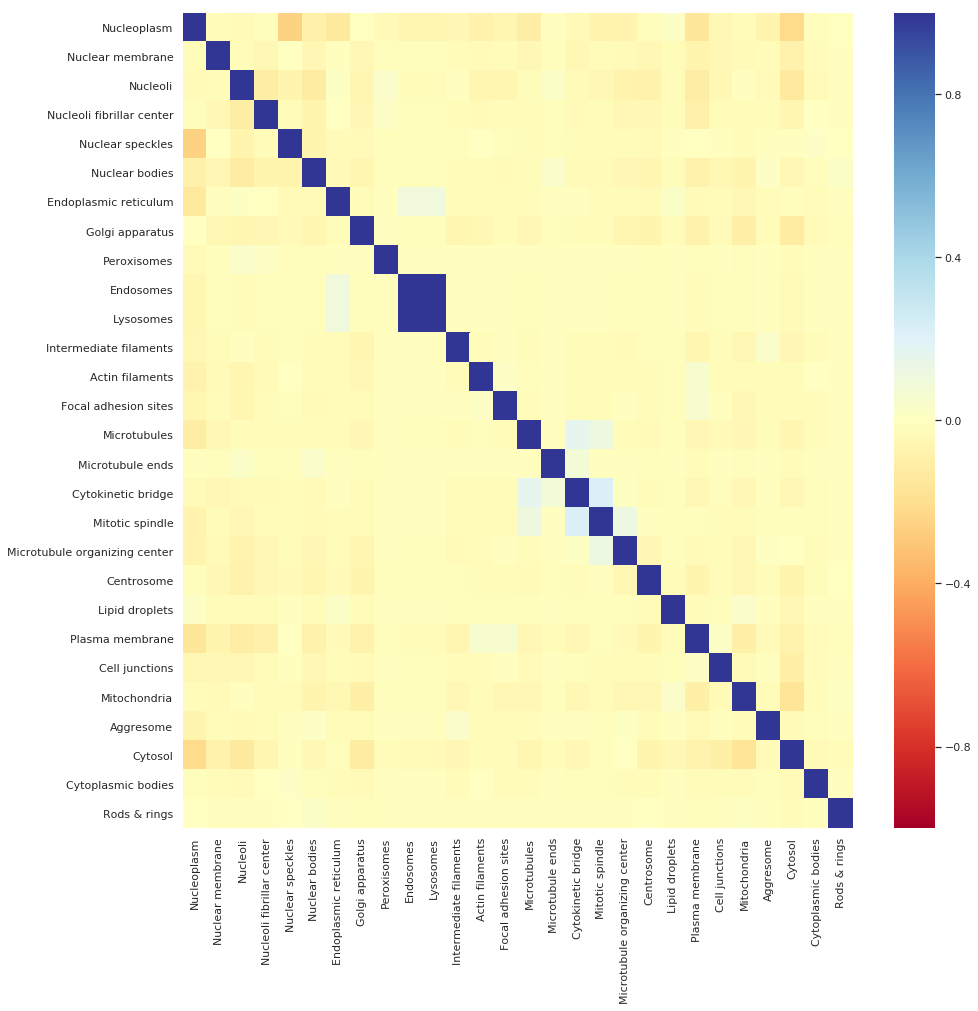
\includegraphics[width=0.8\paperwidth,height=0.8\paperheight]{images/data_analysis_3}
		\end{figure}
	\end{block}
	\end{frame}
	
	\begin{frame}{Data Analysis(3/3)}
	\begin{block}{Highlight Points}
		\begin{itemize}
			\item Data is different from the traditional RGB image.
			\item Data imbalance exists in this dataset.
			\item Some targets are correlated.
			\item Classification results may depend on one or two channels.
		\end{itemize}
	\end{block}
	\end{frame}

%%%%%%%
% Section 2	Method
% Subsection Data Pre-Processing
%%%%%%%
	\subsection{Data Pre-Processing}
	\begin{frame}
	\begin{block}{Affine Transfomation/Histogram Equalization/$\gamma$ Transformation}
		\begin{figure}
			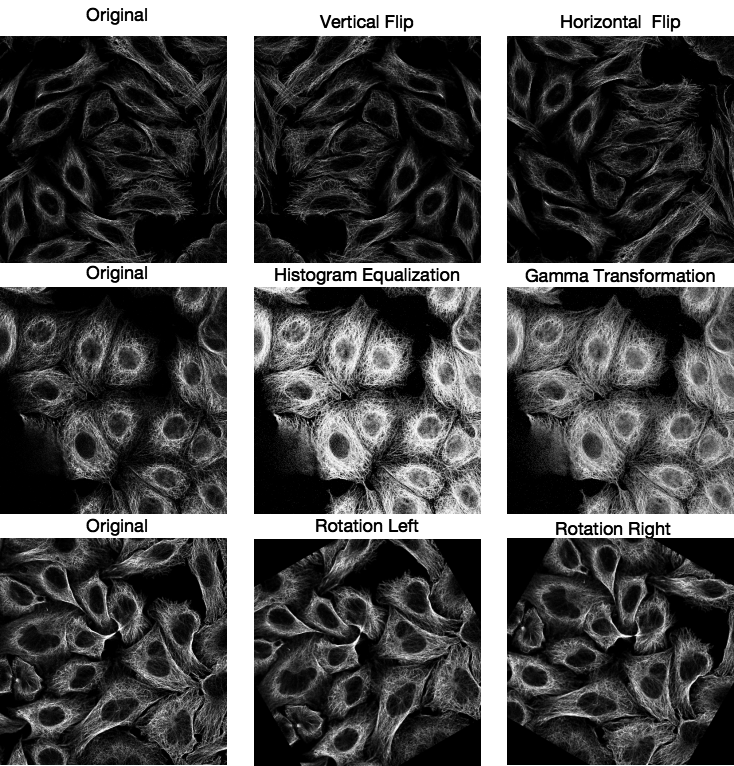
\includegraphics[width=0.6\paperwidth,height=0.8\paperheight]{images/pre_processing}
		\end{figure}
	\end{block}
	\end{frame}

%%%%%%
% Section 2	Method
% Subsection Low level method
%%%%%%%
	\subsection{Low-level Method}
	\begin{frame}
		\begin{columns}
			
		\begin{column}{0.95\paperwidth}
		\begin{block}{SIFT Operator\cite{ng2003sift}}
			Scale Invariant Feature Transform(SIFT) for extracting the keypoints and computing its descriptors.
			\begin{enumerate}
				\item Scale-space Extrema Detection(DoG)
				\item Keypoint Localization
				\item Orientation Assignment
				\item Keypoint Descriptor
				\item Keypoint Matching
			\end{enumerate}
		\end{block}
		\end{column}
%		\begin{column}{0.3\paperwidth}
%		\begin{figure}
%			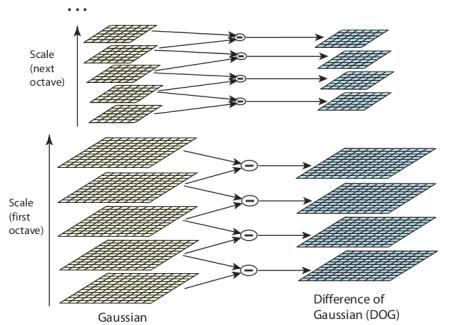
\includegraphics[width=0.3\paperwidth,height=0.3\paperheight]{images/sift_dog}
%		\end{figure}
%		\end{column}
		\end{columns}
		
		\vspace{-6mm}
		\begin{columns}
			
		\begin{column}{0.4\paperwidth}
		\begin{figure}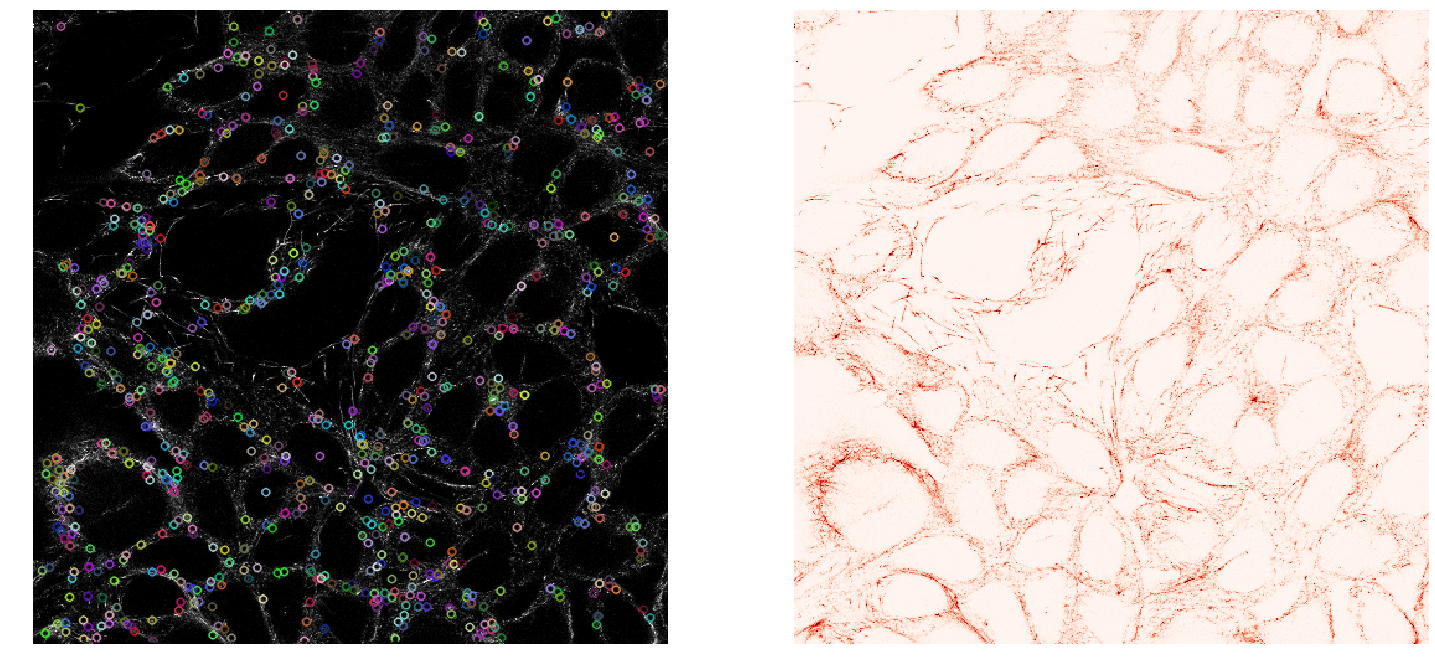
\includegraphics[width=0.5\paperwidth,height=0.3\paperheight]{images/sift_result_0}
		\end{figure}
		\end{column}
		\hspace{8mm}
		\begin{column}{0.4\paperwidth}
		\begin{figure}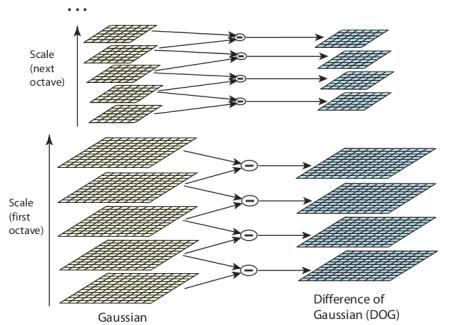
\includegraphics[width=0.4\paperwidth,height=0.4\paperheight]{images/sift_dog}
		\end{figure}
		\end{column}
		\end{columns}
	\end{frame}
	
	\begin{frame}{SIFT+Bag-of-Words\cite{al2016facial,hosmer2013applied}}
	\begin{columns}
	\begin{column}{0.45\paperwidth}
	Step-1: SIFT Keypoint
	\begin{figure}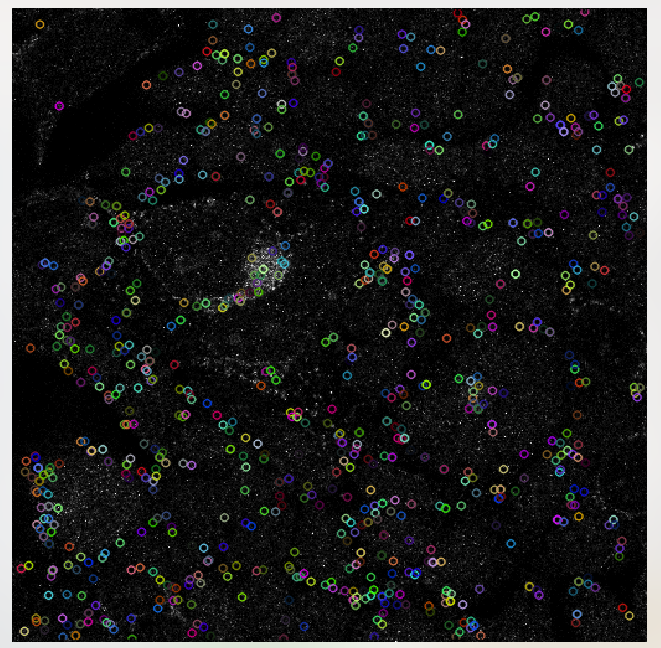
\includegraphics[width=0.25\paperwidth,height=0.25\paperheight]{images/sift_demo}
	\end{figure}
	Step-2: Kmeans to get Dict\cite{basu2002semi}
	\begin{figure}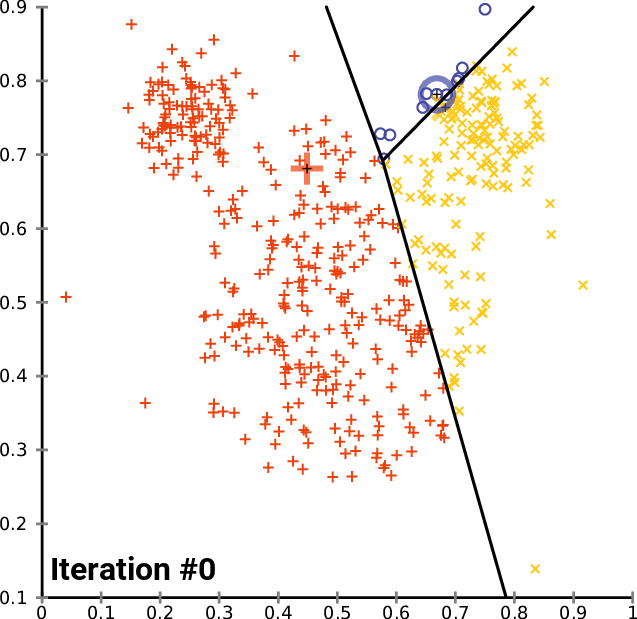
\includegraphics[width=0.3\paperwidth,height=0.3\paperheight]{images/k_means_convergence}
	\end{figure}
	\end{column}
	\begin{column}{0.45\paperwidth}
	Step-3: Get Feature Vector\\
	\begin{figure}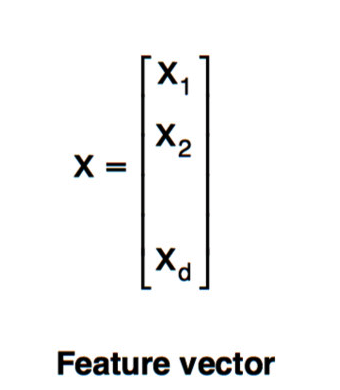
\includegraphics[width=0.2\paperwidth,height=0.3\paperheight]{images/feature_vector}
	\end{figure}
	Step-4: Classification
%	\begin{figure}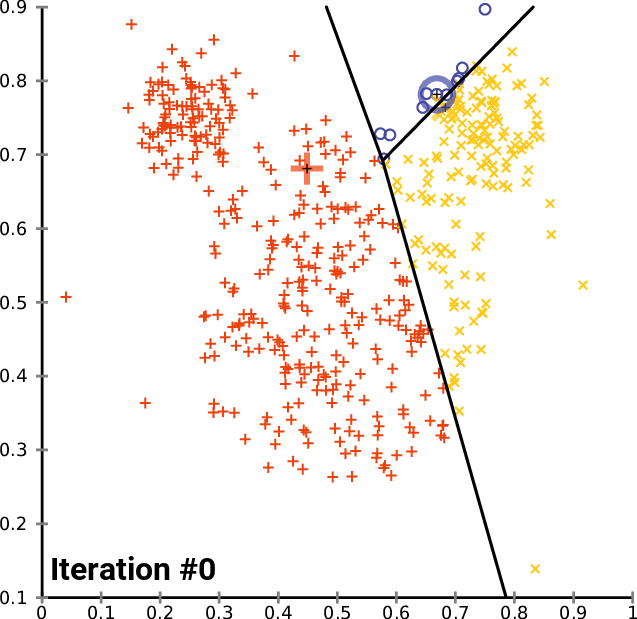
\includegraphics[width=0.3\paperwidth,height=0.3\paperheight]{images/k_means_convergence}
%	\end{figure}
	\end{column}
	\end{columns}
	\end{frame}
%%%%%%
% Section 2	Method
% Subsection DNN-based method
%%%%%%%
	\subsection{DNN-based Method}
	\begin{frame}
		\begin{block}{ResNet34\cite{he2016deep}}
		\begin{figure}
			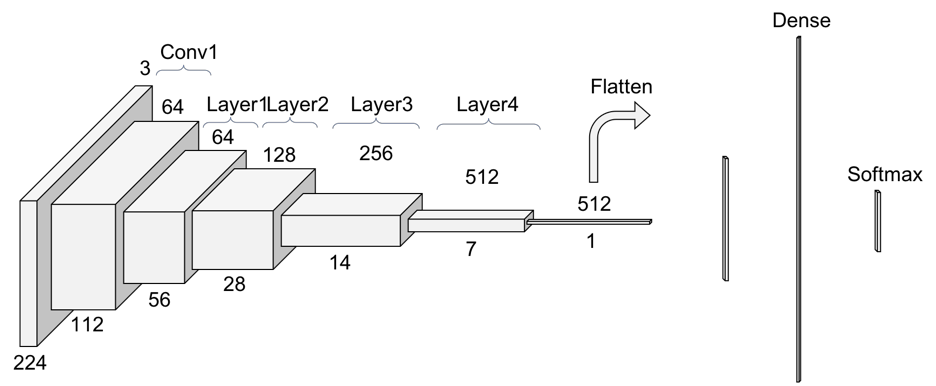
\includegraphics[width=0.8\paperwidth,height=0.4\paperheight]{images/resnet_framework}
		\end{figure}
	\end{block}
	\end{frame}
%%%%%%
% Section 2	Method
% Subsection SIFT-CNN method
%%%%%%%
	\subsection{SIFT-CNN Method}
	\begin{frame}
	\begin{block}{CNN-SIFT Method}
		\begin{figure}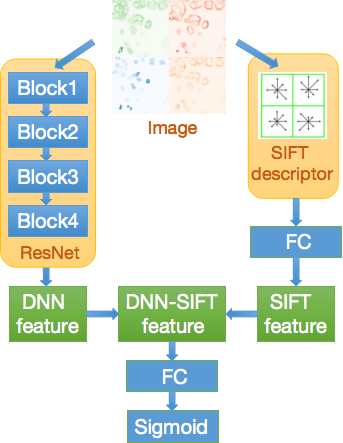
\includegraphics[width=0.5\paperwidth,height=0.8\paperheight]{images/dnn_sift_framework}
		\end{figure}
	\end{block}
	\end{frame}
	
	\section{Experiment}
	\subsection{Quantitive Results}
	\begin{frame}
	\begin{table}[]
		\centering
		 \caption{Results on Human Protein Dataset}
		\label{my-label}
%		\resizebox{\paperwidth}{12mm}{
		\begin{tabular}{|c|c|c|}
			\hline
			&  & Test F1-Score \\ \hline
			\multirow{1}{*}{Low-level Method} & SIFT+Bag-of-Words     & 14.3                \\ \hline 
%			& HOG+Bag-of-Words    & -    \\ \hline
			\multirow{2}{*}{DNN Method}   & ResNet-34    & 37.6    \\ \cline{2-3} 
			   & ResNet-34+PreProcessing & 42.8  \\ \hline
			\multirow{2}{*}{SIFT-CNN Method}& ResNet-34+SIFT & 40.8 \\ \cline{2-3} 
			& ResNet-34+SIFT+PreProcessing &  \textbf{44.5} \\ \hline
		\end{tabular}
	\end{table}
	\end{frame}
%	\subsection{Visualization Results}
%	\begin{frame}
%		
%	\end{frame}
	
	\section{Conclusion}
	\subsection{Summary}
	\begin{frame}
		\begin{block}{Summary}
		\begin{itemize}
			\item Pre-Processing is essential for image classification.
			\item SIFT operator is not as well as DNN-based method.
			\item SIFT and DNN feature are complementary, we can use this strategy to achieve better performance.
			\item F1-Score is good measurement for multi-label classification problem.
			\item Over-sampling\cite{chawla2002smote} or weighted loss are helpful for data imbalance.
		\end{itemize}	
		\end{block}
	\end{frame}
	
	\subsection{Future Research}
	\begin{frame}
		\begin{block}{Feature Work}
		\begin{itemize}
			\item Propose new feature descriptor or network architecture for human protein image.
			\item Explore combining traditional method with learning based method for robust and better performance.
		\end{itemize}	
		\end{block}
	\end{frame}
	
	\subsection{Reference}
	\begin{frame}[allowframebreaks]
        \frametitle{References}
        \bibliographystyle{plain}
        \bibliography{reference.bib}
		
	\end{frame}
\end{document}